
\chapter{Closed Loop LTI Systems} \label{lc_chapter}
%\thispagestyle{fancy}

Consider the closed loop system given by Fig. \ref{chpCLfig01Gcl}.

\begin{figure}[H]
	\centering
	\includegraphics[scale=1.2]{./figuras/chapter_glc/lazocerrado.png}
	\caption{Closed loop LTI system.}
	\label{chpCLfig01Gcl}
\end{figure}


The closed loop system given by Fig. \ref{chpCLfig01Gcl} can be redrawn as presented in Fig. \ref{chp_lc_fig02_GH} for a setpoint change where, according to Adam \cite[see Chap. 9]{Adam2018}, if $G_t(s)=G_m(s)$ the feedback system has a similar behavior that a unity feedback system and consequently it is possible to write, $G(s)=G_p(s)G_v(s)G_m(s)$ y \textit{H}(\textit{s})=\textit{C}(\textit{s}).
\begin{figure}[H]
	\centering
	
\includegraphics[scale=1.2]{./figuras/chapter_glc/fig_GH.png}
	\caption{Closed loop LTI system with unity feedback.}
	\label{chp_lc_fig02_GH}
\end{figure}

For the stability study, remember that it must take into account (Adam, \cite{Adam2018}):

\begin{theorem}[Routh-Hurwitz stability Criterion] \label{teo02_chp_estab}\index{stability!Routh-Hurwitz criterion}
	The necessary and sufficient condition of stability is that all the terms in the first column of the Routh array have the same sign.
\end{theorem}

In this toolbox version, two tools have been developed to allow studying of  stability by mean of the root locus and  Bode and Nyquist stability criteria.

\vspace{0.4cm}
\textbf{Example 3.1.} \label{ejem01_gh_oct}
%\begin{example} \label{ejem01_gh_oct}
Firstly, consider a unity feedback system whose transfer function is presented in Fig. \ref{fig01_ejem01_GH}, with a PI controller where $K_r$ is a variable gain and $T_I=5$. 
\begin{figure}[H]
	\centering
	\includegraphics[scale=1.2]{./figuras/chapter_glc/fig_GH_ejem01.png}
	\caption{Unity feedback system given by Exam. 1.}
	\label{fig01_ejem01_GH}
\end{figure}

The open loop transfer function, \textit{G}(\textit{s})\textit{H}(\textit{s}) results,

\begin{equation}\label{eqn01_ejem01_lc}
	G(s)H(s)=\frac{K_r\cancel{(5s+1)}}{5s}\frac{2}{\cancel{(5s+1)}(s^2+s+1)}=\frac{K^*}{s(s^2+s+1)}
\end{equation}

where for this particular case $K^*=2K_r/5$.

\vspace{0.4cm}
For this example, the closed loop transfer function results,

\begin{equation}\label{eqn02_ejem01_lc}
	\frac{Y(s)}{R(s)}=G_{lc}(s)=\frac{G(s)H(s)}{1+G(s)H(s)}=\frac{K^*}{s^3+s^2+s+K^*}.
\end{equation}

To study the stability of the feedback system,  the Routh stability criterion will be apply based on the characteristic equation of feeback loop system.

Being the characteristic equation of this example, $D(s)=s^3+s^2+s+K^*$ and therefore the Routh array results

\begin{equation*}
	\begin{array} {c|}
		s^3 \\ s^2 \\ s^1 \\ s^0
	\end{array}
	\begin{array} {cc}
		1  & 1 \\
		1  & K^* \\
		1-K^*  & 0  \\
		K^*  & 0 \\
	\end{array}
\end{equation*}

It follows that the system will be \textit{asymptotically stable} if and only if, 0 < \textit{K}* < 1.

\vspace{0.4cm}
Now it is pretended to study the initial and final values reached for a step change in the setpoint \textit{R}(\textit{s}) = \textit{k/s}. To do this, applying the initial value theorem (IVT),
\begin{equation*} 
	y(0^+)= \lim _{s \to \infty} s Y(s) = \lim _{s \to \infty} s \ G_{lc}(s)R(s) =  \lim _{s \to \infty} \cancel{s} \frac{K^*}{s^3+s^2+s+K^*} \frac{k}{\cancel{s}} = 0 ~~\mbox{.}
\end{equation*}

Then, applying the final value theorem (FVT),
\begin{equation*} 
	y(\infty)= \lim _{s \to 0} s Y(s) = \lim _{s \to 0} s \ G_{lc}(s)R(s) = \lim _{s \to 0} \cancel{s} \frac{K^*}{s^3+s^2+s+K^*} \frac{k}{\cancel{s}} =  k
\end{equation*}

From the results of both theorems it is shown that the system starts from zero and reaches the setpoint value. This result is subject to the system being stable in closed loop; this is, 0 < \textit{K}* < 1.

\vspace{0.4cm}
Now adopting \textit{K*} = 0.5 (o sea \textit{Kr} = 1.25) to reach a \textit{GM} = 2, the characteristic closed loop equation results $D(s)=s^3+s^2+s+0.5$ presenting three poles in $s_1= -0.64780$ y $s_{2-3}=-0.17610 \pm j 0.86072$.

Note that both systems do not have zeros.

\vspace{0.4cm}
These results can be easily obtained with the Octave commands,
%------------------------------------------------------------------------------------------------------
% Cargo archivo de Octave para motrar en el ejemplo
%\lstinputlisting[language=Octave,frame=single,firstline=9, lastline=20, caption=Código de Octave del Ejem. \ref{ejem01_glc_oct} para el calculo de las raíces $G(s)H(s)$ y de $G_{lc}(s)$.]{./m/chapter_la/ejem01_lc_ltitool.m}
%------------------------------------------------------------------------------------------------------

\begin{verbatim}
    pkg load control
    
	% G(s)H(s) transfer function
	Kast=0.5;
	s=tf('s');
	GH=Kast/(s*(s^2+s+1));
	
	% G(s)H(s) Poles-Zeros
	polesGH=roots(GH.den{1,1})
	% Closed loop Poles-Zeros
	Gcl=feedback(GH,1)
	polesGcl=roots(Glc.den{1,1})
\end{verbatim}

where the answer in the Octave command window is,
\begin{verbatim}
	polesGH =
	
	-0.50000 + 0.86603i
	-0.50000 - 0.86603i
	0.00000 + 0.00000i
	
	
	Transfer function 'Glc' from input 'u1' to output ...
	
	           0.5
	y1:  -------------------
	     s^3 + s^2 + s + 0.5
	
	Continuous-time model.
	polesGcl =
	
	-0.17610 + 0.86072i
	-0.17610 - 0.86072i
	-0.64780 + 0.00000i
\end{verbatim}

The feedback system step response can be obtained by means of the following Octave command:
\begin{verbatim}
	% Step response
	step(Glc)
\end{verbatim}
that it shown in Fig. \ref{chp_lc_fig01_step_GH}.
\begin{figure}[H]
	\centering
	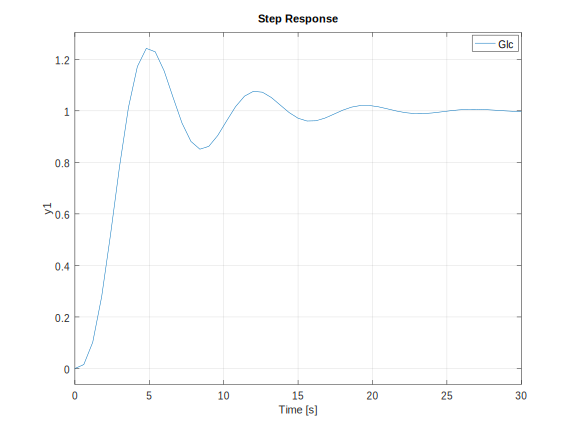
\includegraphics[scale=0.85]{./figuras/chapter_glc/fig01_step_lc.png}
	\caption{Unit step response of the feedback system of the Fig. \ref{fig01_ejem01_GH}.}
	\label{chp_lc_fig01_step_GH}
\end{figure}
%\end{example}



\section{Tools for Feedback LTI Systems}

As mentioned before, two tools for the analysis and simulation of closed loop LTI systems were developed. These ones apply to 
\begin{enumerate}
	\item Feedback system based on \textit{G}(\textit{s})\textit{H}(\textit{s}) according to Fig. \ref{chp_lc_fig02_GH} and,
	\item Closed loop system under the representation of \ref{chp_lc_fig01_lc}.
\end{enumerate}

\subsection{Analysis and Simulation Based on \textit{G}(\textit{s})\textit{H}(\textit{s})}

The tool here developed consists of a function set that allows for a given variable gain value \textit{K}:
\begin{enumerate}
	\item Determine the map of poles and zeros of the transfer function \textit{G}(\textit{s})\textit{H}(\textit{s}) and of the closed loop transfer function with unit feedback for setpoint change.
	\item Present the root locus  of a feedback system, Bode and Nyquist diagrams.
	\item Furthermore, it can also be determined, the dynamic responses of the feedback system given by Fig. \ref{chp_lc_fig02_GH}. For this you must specify,
	\begin{enumerate}
		\item step amplitude and
		\item simulation time
	\end{enumerate}
\end{enumerate}

\vspace{0.4cm}
Besides in this tool, additional information about,
\begin{enumerate}
	\item stability or instability of the feedback linear system;
	\item final value reached by the open loop system once the transient has passed;
	\item Approximated settling time, which is calculated based on the dominant pole(s) of the system. Such calculation can be improved if the simulation time is extended.
	\item The gain value \textit{K*} and the ultimate gain value $K^*_u$ of \textit{G}(\textit{s})\textit{H}(\textit{s}), phase and gain cross frequencies $\omega_{-180}$ and $\omega_{cg}$ respectively; together with the gain and phase margins.
\end{enumerate}

\vspace{0.4cm}
\textbf{Ejemplo 3.2} \label{ejem02_gh_oct}
%\begin{example} \label{ejem02_gh_oct}
As an example, the resolution of the Exam. 3.1 is shown using the developed functions, which can be invoked directly from the Octave command window or, through an .m extension file, as is usually done.

%------------------------------------------------------------------------------------------------------
% Cargo archivo de Octave para motrar en el ejemplo
%\lstinputlisting[language=Octave,frame=single,firstline=14, lastline=55, caption=Código de Octave del Ejem. \ref{ejem01_gla_oct} para el calculo de las raíces de lazo cerrado.]{./m/chapter_lc/auxiliarGHWnd.m}
%------------------------------------------------------------------------------------------------------
\begin{verbatim}
	% packages are loaded.
	pkg load control signal ltitool

	% Clean memory and command window.
	clear all, clc

	% -----------------------------------------------
	% Default values for the variables are defined
	% -----------------------------------------------
	% G(s)H(s):
	s=tf('s');
	Gs=2.0/((5*s+1)*(1*s^2+1*s+1)); delay=0;
	Hs=(5*s+1)/(5*s);
	Kr=1.25;
	GH=minreal(Kr*Gs*Hs);

	% Simulation parameters
	AmplitudSP=1; % step amplitude
	tFinal=30;    % simulation time

	% -----------------------------------------
	% Analisys Tools
	% -----------------------------------------
	% Root locus
	figure(1), clf(figure(1),"reset");
	[Kast,Kast_ult,wultimo,GM,wcg,PM]=GHrlocusplot(GH.num{1,1},GH.den{1,1},Kr,1000);

	% Bode diagrams
	figure(2), clf(figure(2),"reset");
	[Kast,Kast_ult,wultimo,GM,wcg,PM]=GHbodeplot(GH.num{1,1},GH.den{1,1},delay,Kr);

	% Nyquist diagram
	figure(3),  clf(figure(3),"reset");
	[Kast,Kast_ult,wultimo,GM,wcg,PM]=GHnyquistplot(GH.num{1,1},GH.den{1,1},delay,Kr);

	% -----------------------------------------
	% Simulation Tools
	% -----------------------------------------
	% Step response
	figure(4),  clf(figure(4),"reset");
	GHstepresponse(GH.num{1,1},GH.den{1,1},AmplitudSP,tFinal,1000);

	% Impulse response
	figure(5), clf(figure(5),"reset");
	GHimpulseresponse(GH.num{1,1},GH.den{1,1},tFinal,1000);

	% Additional information
	[estabilidad,yinf,Test]=additionalinfo(GH.num{1,1},GH.den{1,1},AmplitudSP,tFinal,1000);
\end{verbatim}

As an example, the root locus diagram of this application is shown.
\begin{figure}[H]
	\centering
	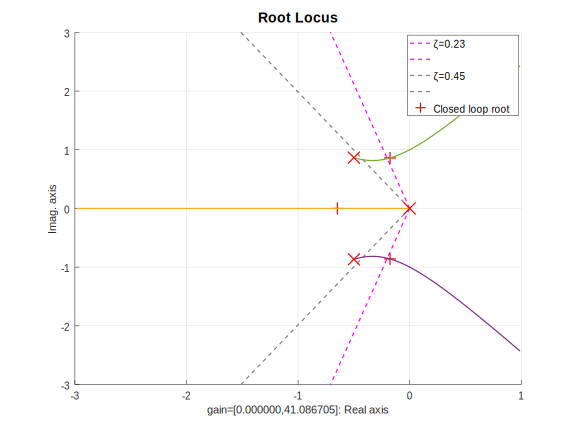
\includegraphics[scale=0.75]{./figuras/chapter_glc/fig_ejem32_GH_ltitool.png}
	\caption{Root locus diagram of Exam. 3.2.}
	\label{chp_lc_fig_LR_ejemGH}
\end{figure}
%\end{example}



\vspace{0.4cm}
\textbf{Ejemplo 3.3}
%\begin{example} \label{ejem03_gh_oct}

Figure \ref{chp_lc_fig01_ejemGH} shows the application window performed for the analysis of closed-loop LTI systems based on the expression of \textit{G}(\textit{s})\textit{H}(\textit{s}).
\begin{figure}[H]
	\centering
	\includegraphics[scale=0.5]{./figuras/chapter_glc/fig01_ejemGH.png}
	\caption{Closed loop system analysis and simulation window based on \textit{G}(\textit{s})\textit{H}(\textit{s}) with preloaded data.}
	\label{chp_lc_fig01_ejemGH}
\end{figure}
Note that the data has been preloaded by a file that saves the data from the last time you worked with this application. There is also a button (Load Default Values Botton) that load the preloaded data for this particular example, which if it pressed, default values are reloaded.

Figure \ref{chp_lc_fig02_ejemGH} shows the numerical simulation of the feedback system when $K^* = 0.5$. Similarly, the poles and zeros maps of \textit{G}(\textit{s})\textit{H}(\textit{s}) can be obtained from the feedback system, together the root locus, Bode and Nyquist diagrams.

In addition, the additional information button provides information of the feedback system related to stability, establishment value, and establishment time, \textit{GM}, \textit{PM}, $\omega_{-180}$ y $\omega_{cg}$. Note that the values $K^*$ and \textit{GM} here reported are coincident with that it was presented by the Exam. 3.1.

\begin{figure}[H]
	\centering
	\includegraphics[scale=0.5]{./figuras/chapter_glc/fig02_ejemGH.png}
	\caption{Closed loop system analysis and simulation window based on \textit{G}(\textit{s})\textit{H}(\textit{s}) with step response.}
	\label{chp_lc_fig02_ejemGH}
\end{figure}
%\end{example}





\subsection{Analysis and Simulation of Feedback System}
In this subsection, it will be considered the closed loop system of Fig. \ref{chpCLfig01Gcl}.


\textbf{Example 3.4}

Figure \ref{chp_lc_fig01_Gcl} shows the developed window for analysis and simulation of closed loop system.

\begin{figure}[H]
	\centering
	\includegraphics[scale=0.5]{./figuras/chapter_glc/fig01_ejemGcl.png}
	\caption{Main window for analysis and simulation of closed loop system.}
	\label{chp_lc_fig01_Gcl}
\end{figure}

Notice that, if the user press load data button then a window like the one in the Fig. \ref{chp_lc_fig02_Gcl} will be present. In it, the data corresponding to the Fig. \ref{chpCLfig01Gcl} must be loaded.


\begin{figure}[H]
	\centering
	\includegraphics[scale=0.5]{./figuras/chapter_glc/fig02_ejemGcl.png}
	\caption{Window for defining of feedback system transfer function.}
	\label{chp_lc_fig02_Gcl}
\end{figure}

On the other hand, the user has a tool for analysis of feedback systems, if the analysis tools button is pressed. Based on the preloaded data in the previous window, this tool provides in a single window with
\begin{enumerate}
	\item Poles-Zeros Map of \textit{G}(\textit{s})\textit{H}(\textit{s}).
	\item Poles-Zeros Map of the feedback system.
	\item Root locus plot
	\item Bode and Nyquist diagrams
\end{enumerate}
as it is shown in Fig. \ref{chp_lc_fig03_Gcl}.

\begin{figure}[H]
	\centering
	\includegraphics[scale=0.5]{./figuras/chapter_glc/fig03_ejemGcl.png}
	\caption{Tool Window for analysis of feedback system.}
	\label{chp_lc_fig03_Gcl}
\end{figure}

Furthermore, the user has a simulation parameter window where allows setting step amplitude and initial time of set-point and disturbance changes and, the simulation time.

\begin{figure}[H]
	\centering
	\includegraphics[scale=0.5]{./figuras/chapter_glc/fig04_ejemGcl.png}
	\caption{Tool window for defining simulation parameters.}
	\label{chp_lc_fig04_Gcl}
\end{figure}


Finally, in Fig. \ref{chp_lc_fig05_Gcl} the simulation of this example is shown.

\begin{figure}[H]
	\centering
	\includegraphics[scale=0.5]{./figuras/chapter_glc/fig05_ejemGcl.png}
	\caption{Window with a simulation example.}
	\label{chp_lc_fig05_Gcl}
\end{figure}


\section{Conclusions}

